%% LaTeX-Beamer template for KIT design
%% by Erik Burger, Christian Hammer
%% title picture by Klaus Krogmann
%%
%% version 2.1
%%
%% mostly compatible to KIT corporate design v2.0
%% http://intranet.kit.edu/gestaltungsrichtlinien.php
%%
%% Problems, bugs and comments to
%% burger@kit.edu

\documentclass[aspectratio=169]{beamer}

%% SLIDE FORMAT

% use 'beamerthemekit' for standard 4:3 ratio
% for widescreen slides (16:9), use 'beamerthemekitwide'

\usepackage{templates/beamerthemekitwide}
% \usepackage{templates/beamerthemekitwide}

\usepackage[utf8]{inputenc}
\usepackage[T1]{fontenc}
\usepackage{lmodern}
\usepackage[ngerman]{babel}
\usepackage{amsmath}
\usepackage{amssymb}
\usepackage{graphicx}
\usepackage{booktabs}
\usepackage{mathabx}
\usepackage{eurosym}
\usepackage{nameref}

%% TITLE PICTURE

% if a custom picture is to be used on the title page, copy it into the 'logos'
% directory, in the line below, replace 'mypicture' with the
% filename (without extension) and uncomment the following line
% (picture proportions: 63 : 20 for standard, 169 : 40 for wide
% *.eps format if you use latex+dvips+ps2pdf,
% *.jpg/*.png/*.pdf if you use pdflatex)

%\titleimage{mypicture}

%% TITLE LOGO

% for a custom logo on the front page, copy your file into the 'logos'
% directory, insert the filename in the line below and uncomment it

%\titlelogo{mylogo}

% (*.eps format if you use latex+dvips+ps2pdf,
% *.jpg/*.png/*.pdf if you use pdflatex)

%% TikZ INTEGRATION

% use these packages for PCM symbols and UML classes
\usepackage{templates/tikzkit}
\usepackage{templates/tikzuml}

\graphicspath{{logos/}, {./images/}}


% the presentation starts here

\title{GIT}
\subtitle{Eine Einführung}
\author[Dominic]{Dominic Heun}
\institute{AES Ettlingen - TGJ2/2}
\date{\today}

% \institute{Chair for Software Design and Quality

\AtBeginSection[]
{
  \begin{frame}
    \begin{center}
    \tableofcontents[currentsection]
    \end{center}
  \end{frame}
}

\begin{document}

  % change the following line to "ngerman" for German style date and logos
  % \selectlanguage{ngerman}

  \setbeamercovered{invisible} % make next text in beamer invisible

  %title page
  \begin{frame}[plain]
    \titlepage
  \end{frame}

  \section{Was ist GIT}

  \begin{frame}{Wie arbeitet man im Team mit eigenen Computern}
    \begin{itemize}[<+->]
      \item Synchronisation?
      \item[$\Rightarrow$] Fehleranfällig \pause mehrere arbeiten gleichzeitig?
      \item[$\Rightarrow$] GIT löst Problem
    \end{itemize}
  \end{frame}

  \begin{frame}{Versionskontrolle}
      \begin{columns}
        \column{0.6\textwidth}

          \begin{itemize}
            \item Verschiedene Versionen
            \item Jeder arbeitet an seinen \textit{Versionen} der Dateien
            \item \textbf{Commit} gibt die Information weiter
            \item \textbf{Merge} fügt die verschiedenen Versionen zusammen
          \end{itemize}

        \column{0.4\textwidth}
          \begin{figure}
            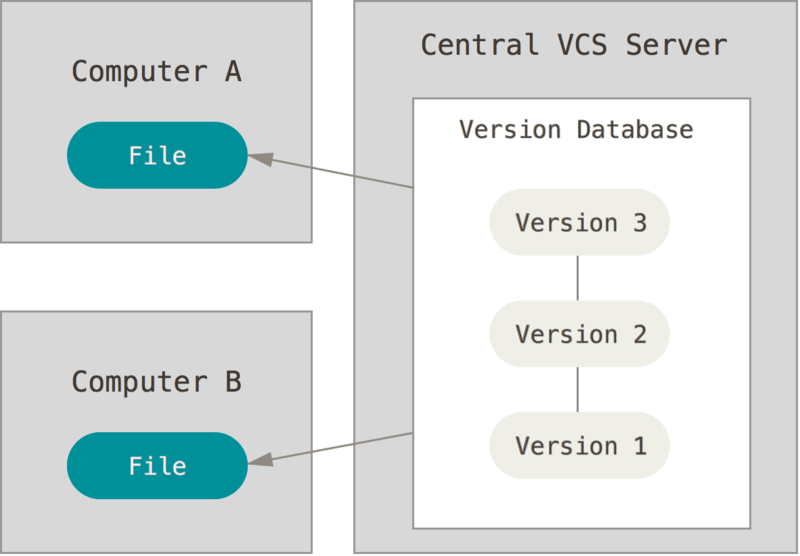
\includegraphics[width=0.9\columnwidth]{version-control-centralized}
            \caption{Versionskontrolle mit zentralem VCS Sever \\
            \tiny{\url{https://git-scm.com/book/en/v2/images/centralized.png}; Abgerufen am 08.05.2018}}
          \end{figure}
      \end{columns}
  \end{frame}

  \section{Git als VCS}

  \begin{frame}{Git}
    \begin{columns}
      \column{0.7\textwidth}
        \begin{itemize}
          \item Eine Möglichkeit unter vielen (\textit{SVN, Git, Mercurial...})
          \item Entwickelt von Linus Torwalds für den \textbf{Linux Kernel}
        \end{itemize}
      \column{0.3\textwidth}
        
\includegraphics[width=0.9\columnwidth]{git}
    \end{columns}
  \end{frame}


\end{document}
